% Source page: Deepfield.md Page 12; exactly one frame.
\setsource{\href{https://doi.org/10.1038/s41551-026-01769-6}{XunZi, Nature (2026)}}
\begin{frame}[c,label=md-12]{XunZi: multi-model data fusion}
\small
\textbf{Motivation:} Reduce hallucinations with multimodal empirical data.
\medskip
\begin{columns}[c,onlytextwidth]
\begin{column}{0.60\textwidth}
    \begin{figure}
    \centering
    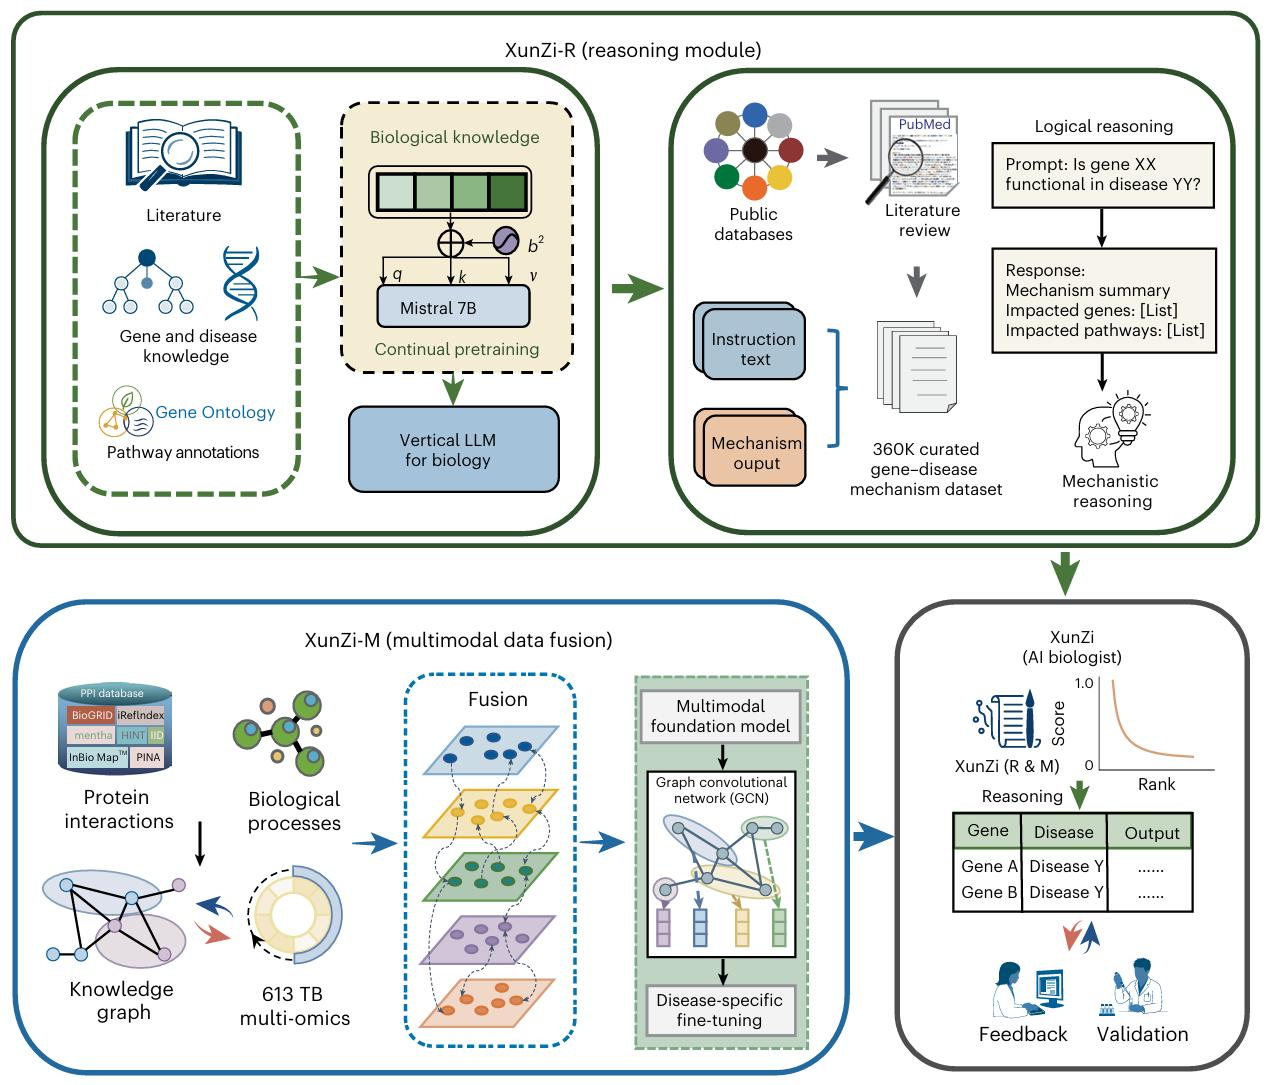
\includegraphics[width=\linewidth,height=4.7cm,keepaspectratio]{architecture_xunzi.png}
    \caption{XunZi architecture}
    \end{figure}
\end{column}
\begin{column}{0.36\textwidth}
    \footnotesize
    \textbf{XunZi-R}\\
    Reasoning model\\[0.25em]
    Continual pretraining\\
    + Supervised fine-tuning
    \medskip

    \textbf{XunZi-M}\\
    GCN fusion model
    \medskip

    \textbf{Dataset}
    \begin{enumerate}
        \setlength{\itemsep}{0.35em}
        \item Publications
        \item Structured biological data
        \item Mechanism CoT\\[0.15em]
        {\footnotesize (manually checked)}
    \end{enumerate}
\end{column}
\end{columns}
\end{frame}

% Source page: Deepfield.md Page 13; exactly one frame.
\setsource{\href{https://doi.org/10.1038/s41551-026-01769-6}{XunZi, Nature (2026)}}
\begin{frame}[t,label=md-13]{XunZi: multi-model data fusion}
\small
\slideheading{XunZi-R: Mistral-7B}
\smallskip
\begin{itemize}
\setlength{\itemsep}{0.3em}
    \item \textbf{CPT:} 24.41M PubMed abstracts + 2.05M structured knowledge records; next-token prediction.
\end{itemize}

\[
\mathcal L_{\rm CLM}=-\sum_{t=1}^T\log P(x_t\mid x_{<t};\theta)
\]
\begin{itemize}
\setlength{\itemsep}{0.3em}
    \item \textbf{SFT:} 330,000 gene--disease mechanism examples.
\end{itemize}

\[
\mathcal L_{\rm SFT}=-\sum_{t=1}^T\log P(y_t\mid y_{<t},x;\theta)
\]
\begin{itemize}
\setlength{\itemsep}{0.3em}
    \item \textbf{Output:} Confidence $s$ for feature fusion, plus a mechanistic explanation for interpretability.
\end{itemize}
\end{frame}

% Source page: Deepfield.md Page 14; exactly one frame.
\setsource{\href{https://doi.org/10.1038/s41551-026-01769-6}{XunZi, Nature (2026)}}
\begin{frame}[t,label=md-14]{XunZi: multi-model data fusion}
\small
\slideheading{XunZi-M: Two-layer GCN}
\smallskip
\begin{itemize}
\setlength{\itemsep}{0.45em}
    \item \textbf{Data:} 2.81M PPI records + 47,900 GO terms; 
    \item \textbf{Graph:} 621,000 nodes and 6.09M edges.
    \item Predict disease-specific gene relevance with binary cross-entropy.
\end{itemize}

\[
\mathcal L_{\rm BCE}=-\sum_{i\in\mathcal Y}
  [y_i\log\hat y_i+(1-y_i)\log(1-\hat y_i)]
\]
\begin{itemize}
\setlength{\itemsep}{0.45em}
    \item \textbf{Output:} Continuous scores in $[0, 1]$ are used to rank candidate targets.
    \item \textbf{Fusion:} Concatenate graph features with $s$; a linear layer produces the final relevance score.
\end{itemize}
\end{frame}

